
    Although validation of a knowledge graph builds on querying, when performed over a SPARQL endpoint, the sections \ref{background_sparql} and \ref{background_shacl} introduced querying and validating a knowledge graph as two different concepts. This section presents the concept of validating SHACL constraints during SPARQL query execution as proposed by Rohde et al. \cite{valSPARQL} as a possibility to improve the validation engine in algorithm \ref{algo:validation_engine}.
    Originally, SHACL constraint validation is done during SPARQL query execution to ``... [increase] the explainability of SPARQL query results by annotating them with information from the SHACL shape schema validation.`` \cite{valSPARQL}.
    Here the inspection of algorithm \ref{algo:validation_engine} shows that the SHACL schema is evaluated over the knowledge graph (line \ref{algo:validation_engine:shaclEngine}) and afterwards combined (lines \ref{algo:validation_engine:start_eval} - \ref{algo:validation_engine:end_eval}) with the query results retrieved before (line \ref{algo:validation_engine:dataset}).
    As shown by Rohde et al., performing both task simultaneously allows to repeatedly exploit the knowledge encoded in the SPARQL query like shown in section \ref{section_shaclapi}.
    
    Next, the notation from section \ref{background_sparql} is extended to perform the SHACL validation from section \ref{background_shacl} during query execution. Afterward, the pseudocode used to repeatedly exploit the knowledge encoded in the seed query $Q_s$ is presented.
    
    In comparison to the notation introduced in \cite{valSPARQL}, the concept of the explanation and the solution mapping is decoupled in a first step and instead there is an explanation function, which is able to map the needed validated RDF terms to a set of validation results. 
    
    \begin{Def}{Explanation Mapping}{valSPARQL_explanation} 
        An explanation mapping $E$ is a partial function, which maps an RDF term $t \in (\mathbf{B} \cup \mathbf{L} \cup \mathbf{I})$ to a set of validation results for that term. A validation result consist of the shape $s \in \mathbf{S}$ against which the node is validated and the validation result, which can be valid ($\top$) or invalid ($\bot$). Therefore it's
        \begin{gather*}
            E: \mathbf{B} \cup \mathbf{L} \cup \mathbf{I} \to \mathcal{P}(\mathbf{S} \times \{\top, \bot\})
        \end{gather*}
        Two explanation mappings $E_1$ and $E_2$ can be united via $E_1 \cup E_2$ by merging the partial functions as follows:
        \begin{gather*}
            E_1 \cup E_2 = \{(t \mapsto E_1(t) \cup E_2(t)) \mid t \in (\mathbf{B} \cup \mathbf{L} \cup \mathbf{I})\}
        \end{gather*}
        where all unspecified values $t$ are assumed to have as default value the empty set.
        The infinite set of explanation mappings is denoted with $\mathbf{E}$.
    \end{Def}
    
    To annotate the query results, it is necessary to extend the notion of a set of solution mappings as introduced in section \ref{background_sparql} with the explanation defined above. 
    
    \begin{Def}{A modified valSPARQL Mapping Set}{valSPARQL_mapping_sets}
    A modified valSPARQL mapping set is a triple $(\Omega, E, sn)$ where $\Omega \subset \mathbf{M}$, $E \in \mathbf{E}$ and $sn \in \mathbf{SN}$.
    \end{Def}    
    
    As in section \ref{background_sparql} several algebraic operations over the solution sets need to be defined. The solution sets are now modified valSPARQL mapping sets instead of sets of SPARQL solution mappings.
     
    \begin{Def}{Algebraic Operations over Modified valSPARQL Mapping Sets}{valSPARQL_algebra}
        Given two modified valSPARQL mapping sets $F_1 = (\Omega_1, E_1, sn_1)$ and $F_2 = (\Omega_2, E_2, sn_2)$, a set of variables $v \subset \mathbf{V}$, a filter condition $R$ and a function used for renaming of variables $\mathcal{r}:\mathbf{V} \to \mathbf{V}$ the following operations are defined:
        \begin{center}
            \begin{tabular}{l|l|l|l}
                \toprule
                operation & $\Omega$ & $\mathcal{G}_E$ & $sn$\\
                \midrule
                \midrule
                $\pi_v(F_1)$ & $\pi_v(\Omega_1)$ & $\{(\mu(x) \mapsto E_1(\mu(x))) \mid x \in v \land \mu \in \Omega\}$ & $sn_1$\\
                $\sigma_R(F_1)$ & $\sigma_R(\Omega_1)$ & $\{(s \mapsto E_1(s)) \mid s \in \text{dom}(\mu) \land \mu \in \Omega \}$ & $sn_1$\\
                $F_1 \cup F_2$ & $\Omega_1 \cup \Omega_2$ & $E_1 \cup E_2$ & $sn_1 \cup sn_2$\\
                $F_1 \bowtie F_2$ & $\Omega_1 \bowtie \Omega_2$ & $E_1 \cup E_2$ & $sn_1 \cup sn_2$\\
                $F_1 \setminus F_2$ & $\Omega_1 \setminus \Omega_2$ & $\{(s \mapsto E_1(s)) \mid s \in \text{dom}(\mu) \land \mu \in \Omega \}$ & $sn_1$\\
                $\rho(\mathcal{r},F_1)$ & $\rho(\mathcal{r}, \Omega_1)$ & $E_1$ & $sn_1$ \\
                \bottomrule
            \end{tabular}
        \end{center} % TODO: Fix the table use \mathcal{G}_{EXP}
        Given the operation in the left most column, the result is a new valSPARQL mapping set $(\Omega, E, sn)$.
    \end{Def}
    
    The next step is to build the explanation mapping during SPARQL query evaluation. 
    
    This is done inductively over the graph pattern expressions and analog to definition \ref{Def:sparql_graph_pattern}. 
    Therefore, the induction starts with the evaluation of a triple pattern, which utilizes a modified version of the entity explanation function defined in \cite{valSPARQL}.
    \begin{Def}{Entity Explanation Function}{valSPARQL_explaination}
    The entity explanation function $\text{exp} : \mathbf{M} \times \mathbf{T} \times  \mathbf{SN} \times \mathbf{G} \to \mathbf{E}$ maps the substituted subject $s$ of a triple pattern $t$, given a mapping $\mu$ to an explanation mapping with respect to the matching shapes $sh \in S$ from a shape schema $sn = (S, \uri{TARG}, \uri{DEF})$ over a knowledge graph $G$. 
    \begin{align*}
        \text{exp}(\mu(t),t,sn,G) =  \{(s \mapsto & \{ (sh, \text{validate}(s,sh,G)) \mid\\ & sh \in S \land s \in [[\uri{TARG}(sh)]]_G\})\}
    \end{align*}
    where $s = \mu(t)[0]$
    \end{Def}
    
    Now the evaluation of a triple pattern with respect to a shape schema and a knowledge graph can be defined as
    
    \begin{gather*}
        [[t]]_G^{sn} = ([[t]]_G, \bigcup_{\mu \in [[t]]_G} \text{exp}(\mu(t), t, sn, G), sn)
    \end{gather*}
    
    The further steps of the induction stay the same as in definition \ref{Def:sparql_graph_pattern} but now use the algebraic operations over the modified valSPARQL mapping sets. Therefore, all occurrences of $[[P]]_G$ in definition \ref{Def:sparql_graph_pattern} need to be replaced with $[[P]]_G^{sn}$ where $sn \in \mathbf{SN}$, $P \in \mathbf{P}$ and $G \in \mathbf{G}$.
        This concludes the notation needed to perform SPARQL query execution during SHACL constraint validation.
    
    \begin{Def}{Execution of $Q$ over $G$ while validating w.r.t. $sn$}{valSPARQL_execution}
        The execution of the SPARQL \uri{SELECT} query $Q$ over the knowledge graph $G$ while validating w.r.t. a shape schema $sn$ is written as a function $[[Q]]_G^{sn}: \mathbf{Q} \times \mathbf{G} \times \mathbf{SN} \to \mathcal{P}(\mathbf{M}) \times \mathbf{E} \times \mathbf{SN}$ and gives a modified valSPARQL mapping set.
    \end{Def}
    
    Finally, to make up the decoupling in the beginning, the query results $\Omega$ can be joined with the modified valSPARQL explanation $E$ to get the annotated query results as in \cite{valSPARQL}:
    \begin{gather}
    \Omega \bowtie E = \{(\{(t, \mu(t)) \mid t \in \text{dom}(\mu)\}, \{(t,sh,val) \mid (sh, val) \in \text{E}(t) \land t \in \text{dom}(\mu)\} ) \mid \mu \in \Omega\} \label{join_mapping_set_validation_results}
    \end{gather}
    Clearly, this step might also be pushed down into the evaluation of the query, which would result in a slight change of definition \ref{Def:valSPARQL_algebra} to handle SPARQL mapping sets joined with the explanation mapping \cite{valSPARQL}. 
        
    The following describes the pseudocode of the valSPARQL approach (algorithm \ref{algo:valSPARQL}).
    The approach decomposes the given query $Q$ into so-called subject star-shaped queries (line \ref{algo:valSPARQL:decomp}), whose results are joined afterwards according to the algebraic operations (see definition 9 in \cite{valSPARQL}) (line \ref{algo:valSPARQL:overall_join}). A subject star-shaped query is a non-nested query consisting of the conjunction of triple patterns with the same subject \cite{vidal2010efficiently}. The pseudocode uses such a decomposition and additionally performs the join (equation \ref{join_mapping_set_validation_results}) per star-shaped query result mapping set (line \ref{algo:valSPARQL:join}). During the decomposition, for each star-shaped query, a shape $s$ is determined. This is done by associating each star-shaped query with a class of entities in the knowledge graph and inferring the shape in the shape schema associated with that class. 
    Besides performing SHACL validation during query processing, also the SHACL schema is reduced as described in section \ref{section_shaclapi} (lines \ref{algo:valSPARQL:reduction_start} - \ref{algo:valSPARQL:reduction_end}). 
    
    \begin{algorithm}[H]
    \caption{Pseudocode of the valSPARQL Approach}\label{algo:valSPARQL}
    \begin{algorithmic}[1]
    \Function{valSPARQL}{Query $Q$, Shape Schema $\mathcal{S}$, Knowledge Graph $G$} 
    	\State $\textit{plan} \gets \textbf{generateBushyExecutionPlan}(Q,\mathcal{S})$ \label{algo:valSPARQL:decomp} \Comment{$ssq$ is a star-shaped query}
    	\ForEach{$(ssq,s) \in \textit{plan}$} \Comment{$s$ is the shape chosen for $ssq$}
    	    \State $sn_i \gets \mathcal{S}$ \label{algo:valSPARQL:reduction_start}
    	    \State $\Phi_{sn_i} \gets \textbf{createDependencyGraph}(sn_i)$
            \State $sn_i.S \gets \textbf{DFS}(\Phi_{sn_i}, s)$
    	    \State $sn_i.\uri{TARG}(s) \gets \uri{SELECT}(?x,id,(ssq \uri{ AND } sn_i.\uri{TARG}(s)))$\label{algo:valSPARQL:reduction_end}
    	    \State $(\Omega_i, E_i, sn_i) \gets [[ssq]]_G^{sn_i}$
    	    \State $M_i \gets \Omega_i \bowtie E_i$ \label{algo:valSPARQL:join}
    	\EndFor
    	\State \Return{$\textbf{applyOperators}(\textit{plan},M_1,...)$} \label{algo:valSPARQL:overall_join}
    \EndFunction
    \end{algorithmic}
    \end{algorithm}
    
    The approach described in this section combines the process of the execution of a SPARQL query with the evaluation of a SHACL schema over a knowledge graph. In the validation engine (algorithm \ref{algo:validation_engine}) the dataset constructing query $Q_D$ is executed without evaluating a SHACL schema. However, the constraints $\mathcal{C}$ are already known and, therefore, one may decide to early evaluate a SHACL schema $\mathcal{S}$ coming from a set of constraints $C \subset \mathcal{C}$ with the target shapes $ts_i$ ($i \in [1,2,...]$) matching the shapes $s$ assigned to the star-shaped queries.
    
    
    
    % Explain the architecture 
    
    % \begin{figure}
    %     \centering
    %     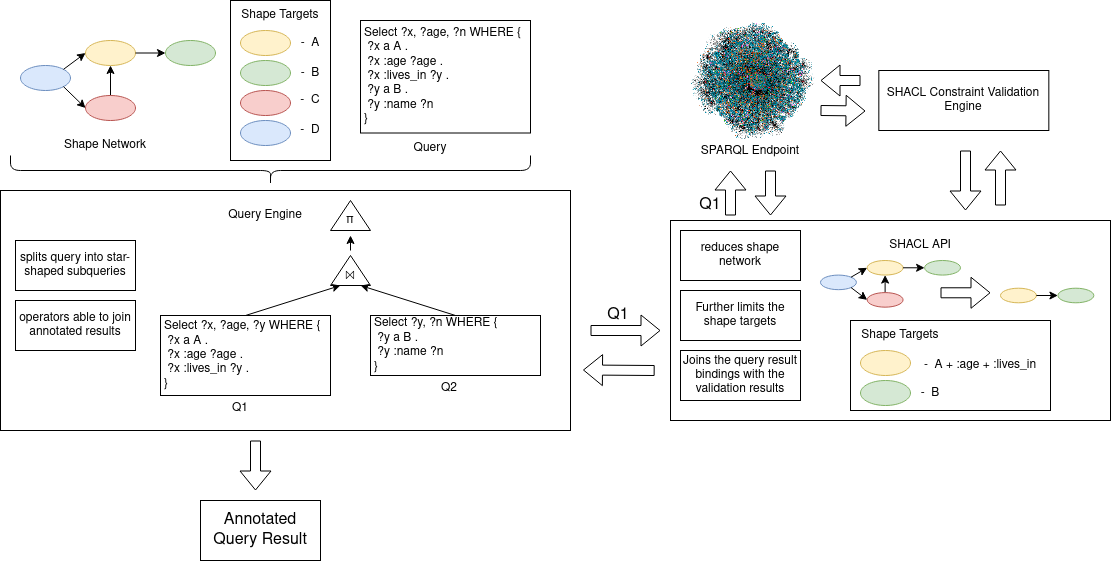
\includegraphics[width=\textwidth]{images/valSPARQL/valSPARQL.png}
    %     \caption{valSPARQL architecture}
    % \end{figure}

    %In general the motivation is twofold. First of all it's something, which is closely related to relational databases. Integrity constraints are defined and checked by the engine (for example a SQL engine) to keep the answers to queries and also the whole database consistent. When querying a possible automated generated knowledge graph, there also might be integrity constraints (then called a shape schema) which should be validated, when accessing the related data. This will then lead to increased explainability of SPARQL query results through annotations with SHACL shape schema validation reports.
    %In the second place with state-of-the art query engines to get validated query results, one would need to evaluate the complete SHACL schema over the graph and then combine the query results with the validation report. Performing both things in parallel leads to space during validation to exploiting the knowledge encoded in the SPARQL query. \cite{valSPARQL}
